% memory reclamation scheme proned to thread failures (unbounded memory leakage)
% DEBRA thread failure for memory reclamation

% they use a ? to get rid of inconsistent experimental results, however for real
% applications, thos inconsistences do exist

% adding works to avoid long run scenarios (low cache miss) -> imporves perf on
% Haswell ?

The authors experimented on several architectures. Some of their experiments are
shown figure \ref{fig:courbe}. They evaluated the MS-Queue (lock-free), CC-Queue
(blocking), LCRQ (lock-free) and their wait-free design named WF-0 (one try on
the fast-path) and WF-10 (10 tries on the fast-path). They also evaluated a
microbenchmark, simulating enqueue and dequeue operations using only one
fetch-and-add. It should serve as an upper bound for any fetch-and-add-based
queue.

Their wait-free queue outperforms most tested designs when run with only one
thread. With several threads, their design performance is close to the lock-free
LCRQ design. Their memory reclamation scheme adds no overhead on x86
architecture, which is unprecedented.

\begin{figure}
  \caption{ Throughput of different queues. A thread decides uniformly at random
    to execute an enqueue or dequeue with equal odds. The benchmark executes
    $10^7$ operations partitioned evenly among all threads. \char`\^:~executions
    that involve multiple processors. \cite{Yang:2016:WQF:3016078.2851168}}
    \label{fig:courbe}
    \center
    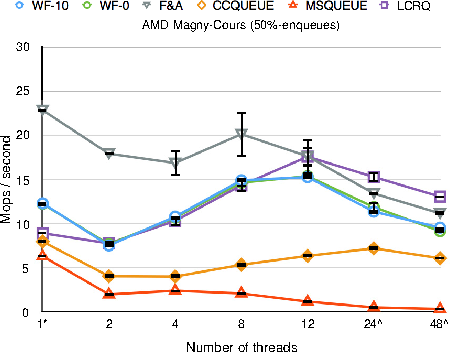
\includegraphics[width=1\linewidth]{img/courbe.pdf}
\end{figure}

In their experiments, the authors haven't compared their queue to another
wait-free queue constructed with the fast-path-slow-path methodology like the
one from A. Kogan and E. Petrank \cite{Kogan:2012:MCF:2370036.2145835}, which
uses MS-Queue as fast-path. The reason given is that this design can only be as
good as the MS-Queue. Because the number of failures of compare-and-swap isn't
bounded for MS-Queue, it is not clear that this wait-free queue can't be faster,
under heavy contention, than the original MS-Queue.

Recent research has suggested that some lock-free objects
\cite{Alistarh:2016:LCA:2997039.2903136} and even blocking objects
\cite{David:2016:CSD:2935764.2935774} can \textit{practically} be considered
wait-free given how unlikely conflicts occur. For example, for the queue
presented in this overview, experimental results show that 99.97\% of the
enqueues and at most 95.95\% of the dequeues are done with only one try on the
fast-path (which is obstruction-free). I believe the research emphasises the
idea that applications needing a state-of-the-art wait-free queue instead of a
simpler, faster obstruction-free or lock-free queue are quite rare.

The authors remind us that fetch-and-add are not universally supported. For
example, the Power, SPARC and ARM processors don't provide a native
fetch-and-add primitive. While it can be emulated with
load-linked/store-conditional primitive, the queue loses its wait-free property.

Fetch-and-add may fail in a similar way as compare-and-swap fails but at
hardware level which blurs the difference between wait-free fetch-and-add-based
queue and lock-free queue. When several fetch-and-add conflict on the same
memory location, I postulate that they must be treated in a starvation-free
manner by the hardware to keep the wait-free property of the queue.

When multiple processors are involved and on architecture where the
fetch-and-add is natively available, the fetch-and-add microbenchmark doesn't
always perform better than the LCRQ which uses fetch-and-swap and
compare-and-swap, as show in figure \ref{fig:courbe} This makes me reconsider
the effectiveness and wait-free property of fetch-and-add.
